\documentclass[preprint,12pt]{elsarticle}

%% for a journal layout:
%% \documentclass[final,1p,times]{elsarticle}
%% \documentclass[final,1p,times,twocolumn]{elsarticle}

\usepackage{orcidlink}

\usepackage{amssymb}
\usepackage{amsmath}
\usepackage{hyperref}
\usepackage{longtable}

%% \begin{linenumbers}, end it with \end{linenumbers}. Or switch it on
%% for the whole article with \linenumbers.
%% \usepackage{lineno}

\journal{Astronomy and Computing}

% Local commands go here.
\newcommand{\docRef}{RTN-091}
\newcommand{\docUpstreamLocation}{\url{https://github.com/lsst/rtn-091}}

\providecommand{\secref}[1]{Section~\ref{#1}}
\providecommand{\appref}[1]{Appendix~\ref{#1}}
\providecommand{\tabref}[1]{Table~\ref{#1}}
\providecommand{\figref}[1]{Figure~\ref{#1}}
\providecommand{\eqnref}[1]{Eq.~\ref{#1}}
\providecommand{\recref}[1]{REC-\ref{#1}}
\def\VRO{Vera C. Rubin Observatory~}
\def\RO{Rubin Observatory~}
\def\aaps{A\&AS}           % Astronomy and Astrophysics Suplement
\def\aap{A\&A}             % Astronomy and Astrophysics
\def\ssr{Space~Sci.~Rev.}  % Space Science Reviews
\def\apj{ApJ}              % Astrophysical Journal
\def\apjs{ApJS}            % Astrophysical Journal Supplement
\def\aj{AJ}                % Astronomical Journal
\def\mnras{MNRAS}          % Monthly Notices of the RAS
\def\araa{ARA\&A}          % Annual Review of Astron and Astrophys
\def\nat{Nature}           % Nature
\def\apjl{ApJ}             % Astrophysical Journal, Letters
\def\icarus{Icarus}        % Icarus
\def\prd{Phys.~Rev.~D}     % Physical Review D
\def\physrep{Phys.~Rep.}   % Physics Reports
\def\pasp{PASP}            % Publications of the Astronomical Society of the Pacific
\def\procspie{Proc.\ SPIE} % Proceedings of the SPIE
\newcommand{\pasa}{PASA}   % Publications of the Astronomical Society of Australia
\newcommand{\ao}{Appl.~Opt.}  % Applied Optics
\def\pasj{PASJ}            % Publications of the Astronomical Society of Japan

\begin{document}

\begin{frontmatter}

%% Title, authors and addresses

\input{authors}
\date{\today}
\title{Rubin at the Summit - observatory cyber infrastructure and security}

% This can write metadata into the PDF.
% Update keywords and author information as necessary.
\hypersetup{
    pdftitle={Rubin at the Summit - observatory cyber infrastructure and security},
    pdfauthor={silvac},
    pdfkeywords={}
}


\begin{abstract}
We describe the modern and dynamic infrastructure as code based system underlying operations of the Vera. C Rubin Observatory. We will also cover or extra efforts to be NIST standard compliant for cyber security.
\end{abstract}


%%Graphical abstract
%\begin{graphicalabstract}
%\includegraphics{grabs}
%\end{graphicalabstract}


\begin{keyword}
Vera C. Rubin Observatory \sep cybersecurity \sep
%% keywords here, in the form: keyword \sep keyword

%% PACS codes here, in the form: \PACS code \sep code
%% or \MSC[2008] code \sep code (2000 is the default)

\end{keyword}

\end{frontmatter}


\section{Introduction}

The Vera C. Rubin Observatory\cite{2019ApJ...873..111I} will go in to operations in 2025.
During commissioning we have already seen our infrastructure as code based cyber system working well.
In this paper we will describe the generic underlying hardware, deployments on that hardware of both bare metal and containerized applications, transmission of data to SLAC and our NIST\cite{NIST.SP.800-171} compliant security approach.

The Rubin summit may be viewed in terms os standard Cyber Infrastructure Layers.
The layers are graphically depicted in \figref{fig:ci-rubin}i which is a revised version of the diagram presented in \cite{2019arXiv190713060O}.
Each layer is covered in a section below as follows:

\begin{enumerate}
\item The physical layer covered in \secref{sec:physical}
\item The network layer covered in \secref{sec:networking}
\item The computing layer covered in \secref{sec:computing}
\item The application layer covered in \secref{sec:application}
\end{enumerate}

\section{Key Considerations}
Before discussing the network infrastructure used for the Rubin Observatory, it is important to understand the conditions under which the Vera C. Rubin Observatory—and most observatories worldwide—operate. 

Observatories typically have two operational sites: one in a city, where offices are located, and another where the actual observatory is situated. This latter site is by far more complex to design and operate.

At Rubin Observatory, we have multiple operational sites. There are two sites in La Serena, one in Tucson, and a data center at Stanford. However, the most challenging site to design, and the one requiring the highest level of precaution, is located on the mountain, one of the two sites in La Serena. This site is not only subject to unique climatic conditions—situated over 2,600 meters above sea level with lower oxygen levels and little humidity—but it is also difficult to access.

Traveling from the nearest city, La Serena, to Cerro Pachón takes approximately two hours. This means that if an urgent issue arises at the observatory—considering problems can occur at any time of day—those two hours must be factored into the response time. If physical intervention is needed and no staff are on-site, the response time could exceed three hours, factoring in the time required for someone to prepare and travel to the location. For any hardware, this delay could be catastrophic. 

Some observatories operate on a shift-based schedule, ensuring someone is always closer to the site, which helps minimize accessibility issues. However, vendors do not maintain the same level of presence near these remote locations as in major cities. As a result, their ability to provide timely support remains constrained by the same logistical challenges of reaching the site.

Therefore, when designing the computing infrastructure of the observatory, the following key conditions had to be considered:

\begin {itemize}
\item Harsh environmental conditions. As a direct consequence, hardware failures are inevitable, making it essential for the observatory to be well-prepared for such incidents.
\item Unreliable power grid. Power outages are almost unavoidable without a dedicated power station near the observatory. 
\item Limited accessibility in urgent situations. The time required for an engineer to reach the site after an alert is triggered must be considered. At Rubin Observatory, this response time is at least three hours, which can be critical for hardware failures. While some observatories mitigate this challenge by implementing shift-based staffing, vendor support remains constrained by the same logistical barriers. As a result, shipping and delivery of replacement parts can take several days.
\item Human factor. The difficulty in accessing the remote site, low oxygen levels, and the pressure to resolve issues quickly can affect the performance of the staff and increase the risk of errors. Therefore, solutions should be as simple as possible, requiring minimal effort and on the spot decision-making from the staff.
\end {itemize}

All these factors were considered in the design of Rubin Observatory's computing infrastructure.

\newpage

\begin{figure}
\begin{centering}
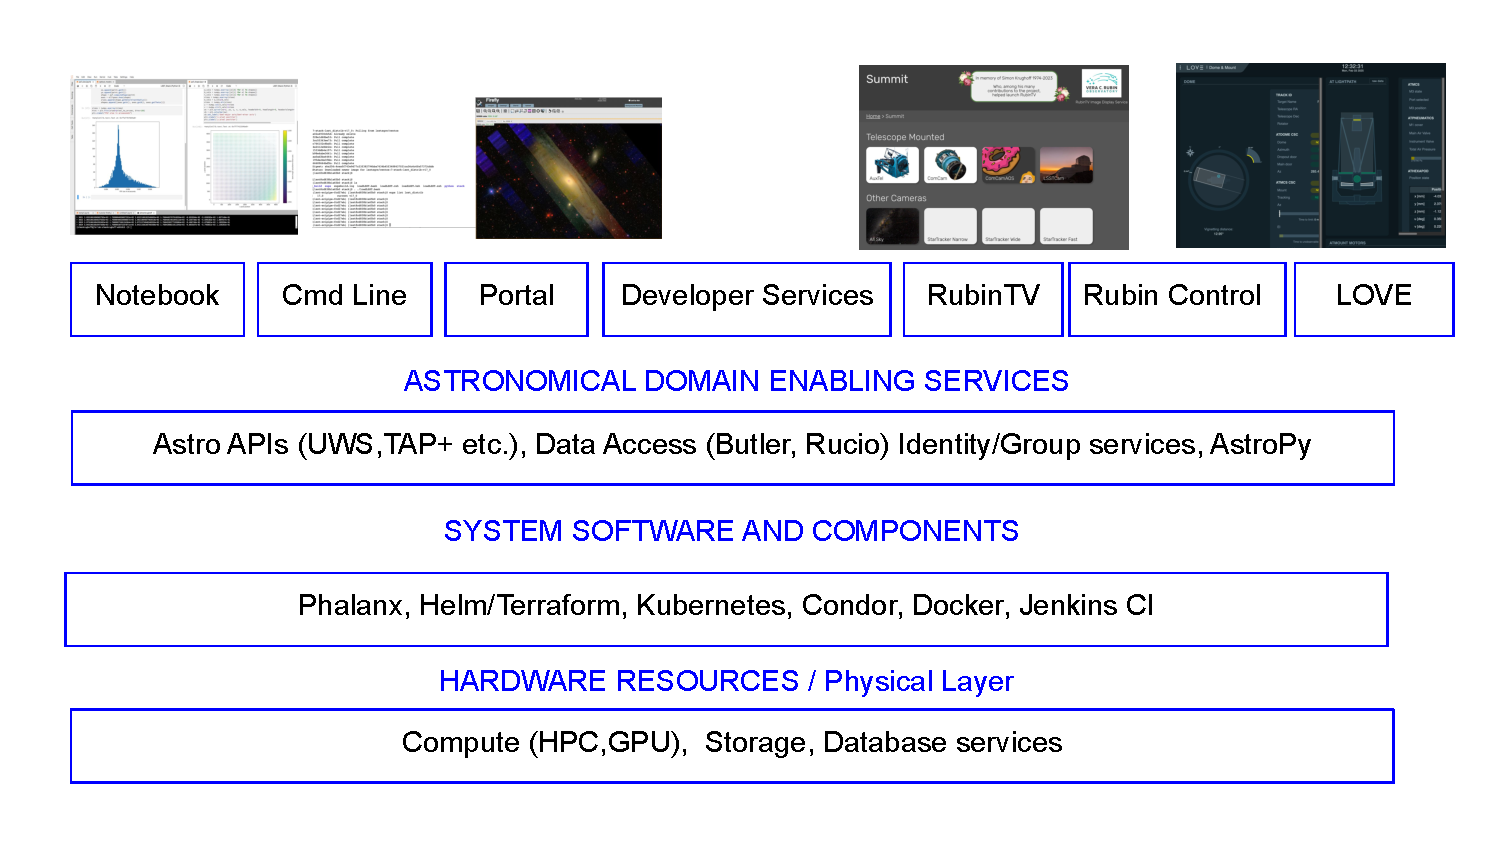
\includegraphics[width=0.9\textwidth]{images/CI-Rubin}
	\caption{Rubin Cyber infrastructure layers
\label{fig:ci-rubin}}
\end{centering}
\end{figure}

\section{Physical Layer} \label{sec:physical}

\subsection{Design}
Scalability, Open design

\subsection{Legos}
Blocks

\section{Networking Layer} \label{sec:networking}

\subsection{Reliability}

\subsection{Scalability}

\section{Computing Layer} \label{sec:computing}

\subsection{Automatizing}
IaC, GitOps, CI/CD

\subsection{Monitoring}
Health, Logs, Dashboards, Alerts

\section{Application Layer} \label{sec:application}

\subsection{Deployments}
Test Stands, Canary, Blue/Green

\subsection{Security}
Detections, Identities, Monitoring

\section{Incidents Management}
Alerts, Escalation,

\section{Documentation}
Technotes, Runbooks



%% Modify acknowldgments as needed.
\textbf{Acknowledgments}\\
This material is based upon work supported in part by the National Science Foundation through Cooperative Agreement AST-1258333 and Cooperative Support Agreement AST-1202910 managed by the Association of Universities for Research in Astronomy (AURA), and the Department of Energy under Contract No. DE-AC02-76SF00515 with the SLAC National Accelerator Laboratory managed by Stanford University.
Additional Rubin Observatory funding comes from private donations, grants to universities, and in-kind support from LSST-DA Institutional Members.




% Include all the relevant bib files so that references can be found from
% lsst-texmf.
% https://lsst-texmf.lsst.io/lsstdoc.html#bibliographies
\bibliographystyle{elsarticle-num}
\bibliography{local,lsst,lsst-dm,refs_ads,refs,books}
\appendix
\input{acronyms.tex}

\end{document}
